\documentclass{standalone}
\usepackage{tikz}

\begin{document}

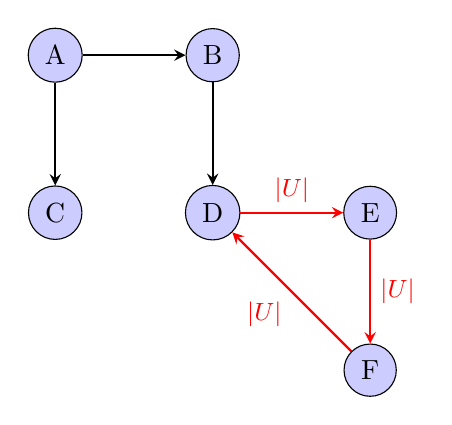
\begin{tikzpicture}[node distance=2cm, auto]

% Define styles for nodes and edges
\tikzstyle{vertex} = [circle, draw, fill=blue!20]
\tikzstyle{edge} = [-stealth, thick]
\tikzstyle{weight} = [font=\small]

% Initial unweighted graph H (blue)
\node[vertex] (A) {A};
\node[vertex] (B) [right of=A] {B};
\node[vertex] (C) [below of=A] {C};
\node[vertex] (D) [below of=B] {D};

\draw[edge] (A) -- node[weight] {} (B);
\draw[edge] (A) -- node[weight] {} (C);
\draw[edge] (B) -- node[weight] {} (D);

% Additional vertices and edges with weight |U| (red)
\node[vertex, right of=D] (E) {E};
\node[vertex, below of=E] (F) {F};
\draw[edge, color=red] (D) -- node[weight, color=red] {$|U|$} (E);
\draw[edge, color=red] (E) -- node[weight, color=red] {$|U|$} (F);
\draw[edge, color=red] (F) -- node[weight, color=red] {$|U|$} (D);

\end{tikzpicture}

\end{document}